\chapterauthor{Marcin Kawalerowicz}
\chapter[Secure Software \ldots]{Secure Software Development Life Cycle: Przegląd Stosowanych Praktyk Bezpieczeństwa}
\thispagestyle{empty}
\vspace{-8mm} {\large Marcin Kawalerowicz} \vspace{8mm}

\section{Wstęp}
Bezpieczeństwo wytwarzania oprogramowania wymaga systematycznego podejścia obejmującego każdą fazę cyklu jego życia - od koncepcji po eksploatację~\cite{Pochu2024}. Współczesne firmy programistyczne implementują Secure Software Development Life Cycle (SSDLC) jako fundament praktyk DevSecOps, integrując kontrole bezpieczeństwa bezpośrednio w potokach CI/CD. Niniejszy przegląd przedstawia aktualne metodologie, narzędzia i standardy stosowane przez organizacje deweloperskie, uwzględniając wymogi NIST, OWASP, CISA Secure by Design oraz specyficzne regulacje europejskie.

Raport z Verizon Data Breach Investigations Report 2025~\cite{Verizon2025} wskazuje na 34\% wzrost wykorzystania podatności w porównaniu z raportem z 2024, podczas gdy badanie stanu DevSecOps przeprowadzone przez Black Duck~\cite{BlackDuck2025} ujawnia, że 81\% DevSecOpsów uważa, iż testy bezpieczeństwa spowalniają rozwój oprogramowania. Te dane podkreślają znaczenie zbalansowanej implementacji SSDLC, która minimalizuje tarcia w zespołach programistycznych przy jednoczesnym zachowaniu wysokiego poziomu bezpieczeństwa wytwarzanego przez nich oprogramowania.

W tym kontekście, skuteczny SSDLC musi łączyć automatyzację z ekspertyzą ludzi, technologie z procesami, oraz zgodność prawa z pragmatyzmem biznesowym.

Na potrzeby tego artykułu użyto czterofazowego modelu SSDLC przedstawionego na rysunki~\ref{fig:ssdlc} obejmującego koncepcję i planowanie, implementację, testowanie oraz wdrożenie i eksploatację.

\begin{figure}
    \centering
    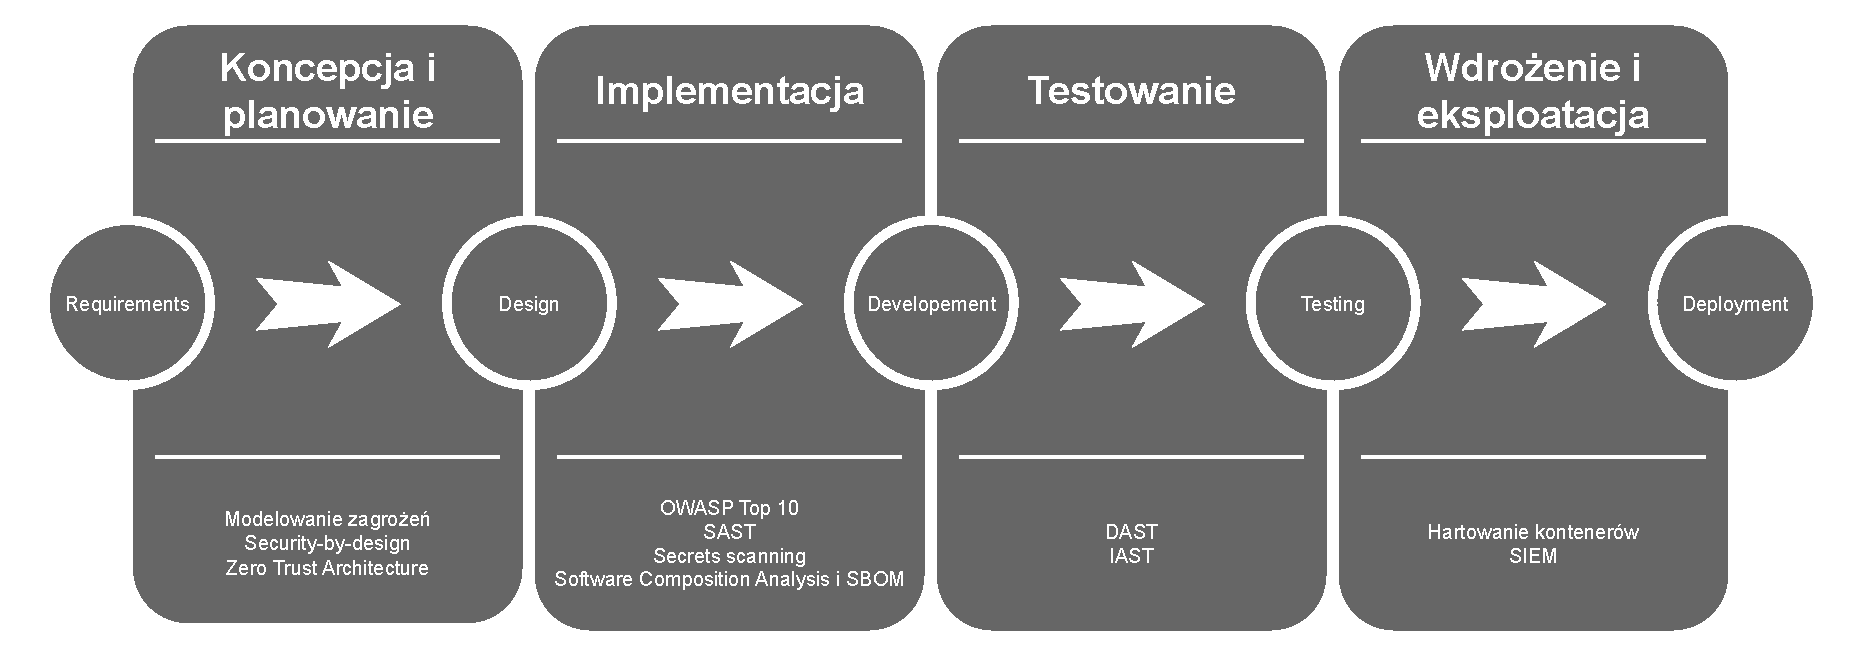
\includegraphics[width=10cm]{fig/ch12/SSDLC.pdf}
    \caption{Model Secure Software Development Life Cycle}
    \label{fig:ssdlc}
\end{figure}

\section{Faza koncepcji i planowania}

\subsection{Metodologie modelowania zagrożeń w praktyce}

Modelowanie zagrożeń stanowi punkt wyjścia dla bezpiecznego projektowania aplikacji. Cztery dominujące metodologie oferują różne podejścia do identyfikacji ryzyk:

\begin{itemize}

\item  STRIDE, zaproponowana przez Microsoft, klasyfikuje zagrożenia według sześciu kategorii:  spoofing (podszywanie się), tampering (modyfikacja), repudiation (zaprzeczenie), information disclosure (ujawnienie informacji), denial of service (odmowa usługi) i elevation of privilege (podniesienie uprawnień). Model ten pozwala identyfikować potencjalne zagrożenia na podstawie diagramów przepływu danych w systemie (Data Flow Diagrams, DFD). Microsoft Threat Modeling Tool to darmowe środowisko do tworzenia modeli opartych na STRIDE.~\footnote{~\url{https://msdn.microsoft.com/en-us/library/ee823878(v=cs.20).aspx}}

\item PASTA (Process for Attack Simulation and Threat Analysis)~\cite{UcedaVelez2015} to siedmiofazowa metodologia zorientowana na ryzyko biznesowe, opracowana przez Tony UcedaVelez i  Marco M. Morana w 2015 roku. Jej kluczową przewagą jest zgodność z celami organizacji oraz symulacja rzeczywistych scenariuszy ataku. PASTA jest rekomendowana dla dużych organizacji, systemów transakcyjnych wysokiej wartości oraz środowisk wymagających zgodności regulacyjnej.

\item LINDDUN~\cite{RoblesGonzalez2020} to ugruntowana metodologia modelowania zagrożeń prywatności, adresująca siedem kategorii: linkability (łączenie), identifying (identyfikacja), non-repudiation (niezaprzeczalność), detecting (wykrywanie), data disclosure (ujawnienie danych), unawareness (brak świadomości) oraz Non-compliance (Nieprzestrzeganie przepisów). Metodologia ta została opracowana przez ekspertów z KU Leuven i jest rekomendowana przez ENISA (Agencję Unii Europejskiej ds. Cyberbezpieczeństwa), a także referencjonowana w opisanym później NIST Privacy Framework.

\item CVSS (Common Vulnerability Scoring System)~\cite{First2019} to standardowa metoda oceny ryzyka oparta na liczbowej skali (0-10), stosowana do oceny wpływu i prawdopodobieństwa zagrożeń.

\item Attack Trees~\cite{Schneier1999} są narzędziem wizualnym, które pomaga zidentyfikować i zorganizować potencjalne ścieżki ataku, umożliwiając analizę skuteczności różnych metod obrony przeciwko tym zagrożeniom. Wizualizują one hierarchicznie ścieżki ataku z węzłami reprezentującymi cele i kroki. Metodologia wspiera analizę what-if dla oceny środków przeciwdziałania i jest często kombinowana z STRIDE oraz CVSS.
\end{itemize}

W tabeli~\ref{tab:threat_modeling_methods} pokazano porównanie wyżej wymienionych metodologii modelowania zagrożeń w oprogramowaniu pod względem 

\begin{table}[ht]
\centering
\caption{Porównanie metodologii modelowania zagrożeń w software}
\label{tab:threat_modeling_methods}
\begin{tabularx}{\textwidth}{*{3}{C}L}
\toprule
\textbf{Metodologia} & \textbf{Fokus} & \textbf{Złożoność} & \textbf{Najlepsze zastosowanie} \\
\midrule
STRIDE & Zagrożenia bezpieczeństwa & Niska-Średnia & Faza projektowania, zespoły początkujące \\
PASTA & Ryzyko biznesowe & Wysoka & Enterprise, compliance, priorytetyzacja ryzyka \\
LINDDUN & Prywatność & Średnia & GDPR/HIPAA, systemy przetwarzające dane osobowe (PII) \\
CVSS & Ocena i klasyfikacja podatności & Niska-Średnia & Ocena ryzyka luk, zarządzanie podatnościami \\
Attack Trees & Ścieżki i scenariusze ataku & Zmienna & Wizualizacja i analiza ścieżek ataku \\
\bottomrule
\end{tabularx}

\end{table}

\subsection{Zero Trust Architecture i Security-by-design}

NIST SP 800-207 to publikacja Narodowego Instytutu Standaryzacji i Technologii (NIST), która określa model Architektury Zero Trust (ZTA), promując zasadę "nigdy nie ufaj, zawsze weryfikuj"~\cite{NIST2020}. Definiuje ona siedem fundamentalnych zasad ZTA:

\begin{enumerate}
\item Wszystkie źródła danych i usługi obliczeniowe traktowane są jako zasoby.
\item Każda komunikacja jest zabezpieczona niezależnie od lokalizacji sieciowej.
\item Dostęp przyznawany jest per-sesja na podstawie dynamicznej polityki.
\item Ciągłe monitorowanie stanu bezpieczeństwa zasobów.
\item Ścisłe egzekwowanie uwierzytelniania i autoryzacji.
\item Kompleksowe logowanie i regularna okresowa ponowna ocena.
\end{enumerate}

Kluczowe komponenty obejmują Policy Decision Point (PDP) oceniający żądania dostępu, Policy Enforcement Point (PEP) jako punkt egzekwujący decyzję o dostępie oraz Policy Engine (PE) implementujący logikę decyzyjną. W kontekście aplikacji, ZTA realizuje się przez API gateways, service mesh oraz otwartego standardu SPIFFE (Secure Production Identity Framework for Everyone)~\footnote{~\url{https://spiffe.io/}} dla tożsamości usług.

Komplementarnym podejściem do ZTA jest inicjatywa CISA Secure by Design~\footnote{~\url{https://www.cisa.gov/securebydesign}}, promująca przeniesienie odpowiedzialności za bezpieczeństwo z użytkowników końcowych na producentów oprogramowania. Model ten opiera się na trzech fundamentalnych zasadach: przejęcie odpowiedzialności za wyniki bezpieczeństwa klientów, transparentność i rozliczalność  oraz budowa odpowiedniej struktury organizacyjnej i przywództwa. Deklaracja Secure by Designe definiuje siedem celów operacyjnych: zwiększenie adopcji wieloskładnikowego uwierzytelniania (MFA), redukcję domyślnych haseł, eliminację klas podatności, przyspieszenie instalacji poprawek, publikację polityk ujawniania podatności, dostarczanie rekordów CVE oraz wdrożenie mechanizmów wykrywania intruzów. Organizacje implementujące Secure by Design powinny traktować bezpieczeństwo jako wymóg na etapie projektowania, nie jako cechę dodawaną po wydaniu oprogramowania.

\section{Faza implementacji}

\subsection{OWASP Top 10 i wytyczne bezpiecznego kodowania}

OWASP Top 10~\footnote{~\url{https://owasp.org/Top10/}} to cyklicznie aktualizowany raport Open Web Application Security Project (OWASP), przedstawiającej dziesięć najważniejszych zagrożeń bezpieczeństwa dla aplikacji internetowych. Dokument ten służy jako standardowy punkt odniesienia dla programistów, testerów i firm, pomagając w identyfikacji krytycznych podatności na podstawie danych o ich powszechności, wykrywalności i wpływie. Lista OWASP Top 10 z 2021 pozostaje autorytatywną wersją z~zapowiedzianą publikacją wersji w tym roku (2025).

\subsection{Narzędzia analizy statycznej kodu źródłowego}

Analiza statyczna kodu źródłowego (Static Application Security Testing, SAST) ma na celu wykrywanie potencjalnych luk bezpieczeństwa, takich jak wstrzykiwanie SQL, podatności typu XSS, fałszowanie żądań po stronie serwera, niepoprawne użycie kryptografii, sekrety w kodzie źródłowym, niebezpieczne deserializacje i~inne. Dobra integracja narzędzi SAST w potoki ciągłej integracji umożliwia szybkie, powtarzalne i wczesne wykrywanie podatności w kodzie, skracając czas reakcji i obniżając koszty napraw.

W kontekście hipotetycznej firmy programistycznej wytwarzającej oprogramowanie głównie w technologii Microsoft .NET (C\#) oraz JavaScript/typeScript, korzystającej z systemu kontroli wersji git (Gitea/GitLab/Bitbucket) oraz systemów CI/CD (Jenkins/Gitlab Pipelines) kluczowe mogą być następujące czynniki wpływające na decyzję o użyciu narzędzi SAST: koszty licencji i utrzymania (preferowane darmowe OSS lub free tier), łatwość integracji z .NET i CI/CD (minimalna konfiguracja), jakość i pokrycie reguł dla C\#/.NET (OWASP Top 10, CVE, frameworki .NET) oraz innych stosowanych języków, wydajność skanowania (czas i zasoby w potokach), możliwość lokalnego uruchamiania (CLI/IDE) przez programistów (opcjonalne), wsparcie i aktywność projektu (community, aktualizacje reguł), zgodność licencyjna i bezpieczeństwo łańcucha dostaw (trusted images, SBOM). Następujące narzędzia SAST zaspokajają te czynniki:

\begin{itemize}
\item  Security Code Scan (SCS)~\footnote{~\url{https://security-code-scan.github.io}}. Charakterystyka: zestaw reguł Roslyn dla C\#/.NET, integracja jako pakiet NuGet/analyzer; działa w IDE, dotnet build i CI; OSS. Zalety: niski koszt (OSS), prosta integracja (NuGet), natychmiastowy feedback w IDE, reguły pod OWASP/CWE, łatwe egzekwowanie w CI (traktowanie ostrzeżeń jako błędy). Wady: brak aktualizacji (ostatnie wydanie ~2022), zgłoszone problemy ze zgodnością (.NET 8+), węższe pokrycie i mniejsze tempo aktualizacji reguł.
\item SonarQube/SonarCloud (reguły Security + Quality)~\footnote{~\url{https://www.sonarsource.com/open-source-editions/}}. Zalety: bogate raportowanie, reguły security i code quality, bramki jakości, integracje CI. Wady: koszt (pełne reguły security w edycjach płatnych), wymagany serwer (self-host) lub subskrypcja; dodatkowa konfiguracja.
\item Semgrep~\footnote{~\url{https://semgrep.dev/}}. Zalety: szybki, reguły konfigurowalne, darmowy core i darmowe reguły community, SARIF, łatwa integracja w CI, aktywnie rozwijany; wsparcie wielu języków i rodzajów plików (np. Dockerfile). Wady: część reguł wymaga dostrojenia pod kontekst projektu; pokrycie .NET stale rośnie, ale nie zawsze dorównuje narzędziom komercyjnym. 
\item Snyk~\footnote{~\url{https://snyk.io/}}. Zalety: Narzędzie typu all-in-one do SCA, SAST, CI/CD, kontenery. Wady: opłaty licencyjne, black-box (trudno konfigurowalny), mniejsza liczba reguł SAST
\end{itemize}

\subsection{Secrets scanning}

Wykrywanie wycieków sekretów w kodzie źródłowym jest ważnym elementem bezpiecznego DevSecOps, zapobiegającym przypadkowemu ujawnianiu kluczy API, haseł czy tokenów w repozytoriach Git. Wielowarstwowe podejście z narzędziami takimi jak Gitleaks czy TruffleHog pozwala na szybkie wykrywanie i blokowanie wysyłania zmian, minimalizując ryzyko wykorzystania luk bezpieczeństwa.

Narzędzia do skanowania sekretów w kodzie źródłowym:

\begin{itemize}
\item Gitleaks~\footnote{~\url{https://gitleaks.io/}}. Najlepsze wyniki w wielu benchmarkach dzięki szybkości i~niskim poziomie fałszywych alarmów. Jest szybki, lekki i dobrze nadaje się do CI/CD.

\item TruffleHog~\footnote{~\url{https://trufflesecurity.com/}}. Oferuje entropy analysis + pattern matching oraz skanowanie rpozytoriów Git, S3 buckets, Confluence, Slack i innych. 

\item GitGuardian~\footnote{~\url{https://www.gitguardian.com/}}. Bezpłatny bazujący na CLI ggshield dla indywidualnych użytkowników oraz komercyjna platforma dashboardem i validity checks.

\item GitHub Secret Scanning~\footnote{~\url{https://docs.github.com/en/code-security/secret-scanning}}. Skanuje kod w poszukiwaniu sekretów i zapewnia push protection – blokowanie prób wysłania wrażliwych danych do repozytorium. W przypadku wykrycia tokenu GitHub powiadamia odpowiedniego dostawcę w celu jego unieważnienia. 

\item GitLab Secret Detection~\footnote{~\url{https://docs.gitlab.com/user/application_security/secret_detection/}} wykorzystuje wewnętrznie Gitleaks z opcją Secret Push Protection.
\end{itemize}

\subsection{Software Composition Analysis i SBOM}

Software Composition Analysis (SCA) oraz Software Bill of Materials (SBOM) umożliwiają identyfikację i zarządzanie komponentami open source w aplikacjach, minimalizując ryzyka podatności i naruszeń licencyjnych w łańcuchu dostaw oprogramowania~\cite{Prana2021}. Formaty SBOM:
\begin{itemize}
\item SPDX (ISO/IEC 5962:2021) to międzynarodowy standard oferujący kompleksowe metadane skupione na zgodności licencyjnej oprogramowania.
\item SPDX 3.0 wydany w kwietniu 2024, wprowadza specjalizowane profile ułatwiające zastosowanie standardu w konkretnych przypadkach użycia, takich jak bezpieczeństwo, kompilacja oprogramowania, sztuczna inteligencja oraz zestawy danych.
\item CycloneDX (OWASP) to format SBOM o priorytecie bezpieczeństwa, oferujący natywne wsparcie dla VEX (Vulnerability Exploitability eXchange) do oceny podatności, podpisy cyfrowe dla integralności oraz identyfikację komponentów poprzez Package-URL (PURL).
\end{itemize}

Narzędzia generujące SBOM:
\begin{itemize}
\item Syft~\footnote{~\url{https://anchore.com/platform/sbom/}} biblioteka Go i narzędzie CLI do generowania CycloneDX/SPDX, zawiera CPE (Common Platform Enumeration).
\item Trivy~\footnote{~\url{https://www.aquasec.com/products/trivy/}} to wszechstronny skaner all-in-one do wykrywania podatności, błędów konfiguracji, sekretów oraz generowania SBOM.
\item cdxgen~\footnote{~\url{https://owasp.org/www-project-cdxgen/}} oficjalny generator CycloneDX od OWASP; posiada profile dla różnych przypadków użycia.
\end{itemize}

\section{Faza testowania}

Faza testowania w procesie bezpiecznego wytwarzania oprogramowania koncentruje się na zautomatyzowanych metodach wykrywania podatności bezpieczeństwa (DAST i IAST), które można wbudować w potok ciągłej integracji i dostarczania~\cite{Abdiukov2024}. 

Świadomie pominięto tutaj zagadnienia związane z testami penetracyjnymi (penetration testing) oraz testowaniem fuzz (fuzz testing), które mimo istotnej roli w ocenie bezpieczeństwa wykraczają poza zakres zautomatyzowanych mechanizmów kontroli możliwych do wdrożenia w standardowych procesach deweloperskich. Testy penetracyjne wymagają specjalistycznej wiedzy i są zazwyczaj są przeprowadzane okresowo przez dedykowane zespoły, podczas gdy fuzz-testing, choć możliwy do zautomatyzowania, stanowi wysoce wyspecjalizowaną dziedzinę wymagającą odrębnego omówienia.

\subsection{DAST}

DAST (Dynamic Application Security Testing) to testowanie bezpieczeństwa typu black-box działającej aplikacji, symulujące rzeczywiste ataki zewnętrznego napastnika bez dostępu do kodu źródłowego. Metoda ta identyfikuje podatności w~środowisku wykonawczym takie jak XSS, SQL injection czy błędy konfiguracji, idealnie integrując się z CI/CD. Narzędzia DAST:

\begin{itemize}
\item OWASP ZAP~\footnote{~\url{https://www.zaproxy.org/}} to najpowszechniej używany skaner z funkcjami Spider Module, AJAX Spider (headless Chromium), Active/Passive Scanning oraz API Scanning (OpenAPI/Swagger). Integracja CI/CD przez obraz Dockera, plugin do Jenkinsa lub GitHub Actions. 

\item Burp Suite DAST~\footnote{~\url{https://portswigger.net/burp/dast}} oferuje skanowanie oparte na przeglądarce, testowanie bezpieczeństwa poza OAST (Out-of-band Application Security Testing), ponad 250 rozszerzeń oraz skalowalne skanowanie wielu aplikacji jak również wsparcie dla uwierzytelniania wieloskładnikowego (MFA), wersję hostowaną w chmurze oraz skanowanie podatności w~protokole WebSocket.

\item Nuclei~\footnote{~\url{https://projectdiscovery.io/nuclei}} to skaner oparty na szablonach prowadzony przez społeczność (w~tym wiele szablonów dla CVE). Oferuje mniej fałszywych alarmów dzięki symulacji warunków rzeczywistych. Posiada aktualizacje społecznościowe. Obsługiwane protokoły: HTTP, DNS, TCP, SSL, WHOIS, JavaScript.
\end{itemize}

\subsection{IAST}

IAST (Interactive Application Security Testing) to hybrydowa metoda testowania bezpieczeństwa, instrumentująca aplikację sensorami w runtime, co łączy analizę statyczną kodu z dynamicznym monitorowaniem przepływu danych i wykonania podczas interaktywnych testów. Ma zapewniać wyższą precyzję przez kontekst na poziomie kodu w środowiskach CI/CD i QA. Wymaga integracji z aplikacją (Java, .NET, Node.js itp.).

\begin{itemize}
    \item OWASP Noir~\footnote{~\url{https://owasp.org/www-project-noir/}} narzędzie IAST wspomagające DAST poprzez statyczną analizę kodu źródłowego.

\item Contrast Security~\footnote{~\url{https://www.contrastsecurity.com/glossary/interactive-application-security-testing}} oferuje instrumentację agentową zwiększając wskaźnik wykrywlności. Wspiera Java, .NET, Node.js, Python, Ruby, Go.

\item Black Duck Seeker~\footnote{~\url{https://www.blackduck.com/interactive-application-security-testing.html}} rozwiązanie z aktywną weryfikacją i śledzeniem danych wrażliwych dla aplikacji webowych, automatyzujące testy bezpieczeństwa dla zespołów deweloperskich.
\end{itemize}

\section{Faza wdrożenia i eksploatacji}

Faza wdrożenia i eksploatacji stanowi moment, w którym aplikacja trafia do środowiska produkcyjnego i staje się dostępna dla użytkowników końcowych oraz potencjalnych napastników.

\subsection{Hartowanie kontenerów}

Obrazy kontenerów mogą zawierać podatności w bibliotekach i zależnościach, znane luki bezpieczeństwa (CVE) w obrazach bazowych, przypadkowo osadzone sekrety (klucze API, hasła, tokeny) oraz błędy konfiguracji. Hartowanie kontenerów (conainter hardening) zapewnia systematyczne skanowania podatności w~kontenerach

Narzędzia takie jak Trivy (opisany w skecji dotyczącej SBOM) oferują kompleksową analizę obejmującą wykrywanie podatności w zależnościach dla ponad 20 menedżerów pakietów (w tym npm, yarn, NuGet), detekcję wycieków sekretów, analizę plików Dockerfile oraz generowanie SBOM w~formatach SPDX i~CycloneDX, integrując się natywnie z potokami CI/CD i rejestrami obrazów.

Bezpieczeństwo kontenerów w środowisku produkcyjnym rozciąga się również na warstwę orkiestracji, gdzie Kubernetes wprowadza dedykowane mechanizmy kontroli w postaci Pod Security Standards (PSS)~\footnote{~\url{https://kubernetes.io/docs/concepts/security/pod-security-standards/}}. Egzekwowanie polityk bezpieczeństwa na poziomie klastra realizowane jest przez silniki takie jak OPA/Gatekeeper wykorzystujący język Rego dla złożonych reguł lub Kyverno oferujący prostszą składnię opartą na natywnym YAML, zapewniając automatyczną weryfikację zgodności wdrażanych zasobów z organizacyjnymi standardami bezpieczeństwa.

\subsection{SIEM}

Monitoring bezpieczeństwa i zarządzanie incydentami (Security information and event management, SIEM) tworzą zamknięty cykl wykrywania, analizy i remediacji zagrożeń poprzez analizę w czasie rzeczywistym alertów bezpieczeństwa generowanych przez aplikacje i sprzęt sieciowy. Rozwiązania typu SIEM:

\begin{itemize}
\item Splunk Enterprise Security~\footnote{\url{https://www.splunk.com/en_us/products/enterprise-security.html}} ma ponad 1500 integracji, zaawansowana naliza, język zapytań SPL
\item Microsoft Sentinel~\footnote{~\url{https://www.microsoft.com/pl-pl/security/business/siem-and-xdr}} jest zbudowany dla ekosystemu chmurowego Azure, wykrywanie zagrożeń oparte o AI/ML, język zapytań KQL
\item Elastic Security~\footnote{~\url{https://www.elastic.co/security}}: integracja ze stackiem ELK, wysoce skalowalny, otwartoźródłowy
\item Wazuh~\footnote{~\url{https://wazuh.com/}}: Open source, schematy zgodności z HIPAA/PCI-DSS, mozliwość dosotoswania do potrzeb
\end{itemize}

\section{Wnioski i dalsze kroki}

Skuteczna implementacja Secure Software Development Life Cycle w organizacjach deweloperskich wymaga zbalansowanego podejścia łączącego automatyzację z ekspertyzą ludzką. Strategia shift-left security~\cite{Malik2025} realizowana przez integrację narzędzi SAST/SCA w potokach CI/CD (Semgrep, Snyk, Security Code Scan, Gitleaks) umożliwia wczesne wykrywanie podatności przy minimalnym wpływie na przepustowość zespołów deweloperskich. Wielowarstwowa ochrona sekretów stanowi fundament dla zapobiegania wyciekom danych uwierzytelniających. SBOM jako ciągła praktyka wymaga utrzymywania SBOM zsynchronizowanego z rzeczywistym stanem zależności w produkcji. 

Przyszłe prace powinny skupić się na trzech kluczowych obszarach wymagających pogłębionej analizy empirycznej i rozwiązań technologicznych:

\begin{itemize}
\item Wspomagana AI Security Code Review i wykrywanie podatności w~oparciu o modele językowe.
\item Zautomatyzowane testowanie bezpieczeństwa dla architektur cloud-native.
\item Weryfikacja bezpieczeństwa łańcucha dostaw.
\end{itemize}

\begin{thebibliography}{30}

\bibitem{Pochu2024}
Pochu S., Kathram S.R.,
Integrating Security Requirements Into Software Development: A Comprehensive Approach to Secure Software Design,
Journal for Multidisciplinary Research, Vol. 1, No. 03, 60--76 (2024).

\bibitem{Verizon2025}
Verizon,
2025 Data Breach Investigations Report,
Verizon Business, https://www.verizon.com/business/resources/reports/dbir/ (2025).

\bibitem{BlackDuck2025}
Black Duck,
The Global State of DevSecOps: Balancing AI Usage and Risk in 2025,
Black Duck Software, Inc., 
https://www.blackduck.com/content/dam/black-duck/en-us/reports/rep-global-devsecops-report.pdf (2025).

\bibitem{UcedaVelez2015}
UcedaVelez T., Morana M.M.,
Risk Centric Threat Modeling: Process for Attack Simulation and Threat Analysis,
Wiley Publishing (2015).

\bibitem{RoblesGonzalez2020}
Robles-González A., Parra-Arnau J., Forné J.,
A LINDDUN-Based framework for privacy threat analysis on identification and authentication processes,
Computers \& Security, Vol. 94, 101755 (2020).

\bibitem{Schneier1999}
Schneier B.,
Attack Trees,
Dr. Dobb's Journal, 
https://www.schneier.com/academic/archives/1999/12/attack\_trees.html (December 1999).

\bibitem{First2019}
FIRST (Forum of Incident Response and Security Teams),
Common Vulnerability Scoring System: Specification Document,
FIRST.org (2019).

\bibitem{NIST2020}
Rose S., Borchert O., Mitchell S., Connelly S.,
Zero Trust Architecture,
NIST Special Publication 800-207,
doi: 10.6028/NIST.SP.800-207,
National Institute of Standards and Technology (August 2020).

\bibitem{Prana2021}
Prana G.A.A., Sharma A., Shar L.K., Foo D., Santosa A.E., Sharma A., Lo D.,
Out of sight, out of mind? How vulnerable dependencies affect open-source projects,
Empirical Software Engineering, Vol. 26, No. 4, 59,
doi: 10.1007/s10664-021-09959-3 (2021).

\bibitem{Abdiukov2024}
Abdiukov T.,
Automated security testing in DevSecOps pipelines: Integrating AI-based vulnerability discovery and compliance validation,
World Journal of Advanced Research and Reviews, Vol. 22, No. 01, 2083--2093,
doi: 10.30574/wjarr.2024.22.1.1083 (2024).

\bibitem{Malik2025}
Malik G., Prashasti P.,
Shift Left Security,
The Eastasouth Journal of Information System and Computer Science, Vol. 2, No. 03, 219--245,
doi: 10.58812/esiscs.v2i03.528 (2025).

\end{thebibliography}
